\documentclass[12pt]{article}

\usepackage{amssymb,amsmath,amsfonts, booktabs, dsfont, eurosym,float,geometry,ulem,graphicx,caption,color,setspace,sectsty,comment,footmisc,caption,multicol, multirow, natbib, pdflscape,array,hyperref}
\bibliographystyle{rusnat}


\normalem



\begin{document}



\begin{titlepage}
\title{Eviction and Crime: Evidence from Boston}
\author{Arjun Shanmugam}
\date{\today}
\maketitle
\begin{abstract}
\noindent This paper investigates the effects of eviction on the frequency of crime incident responses in the immediate vicinity of a property. I use a difference-in-differences research design based on the staggered conclusion of eviction cases in Boston, Massachusetts between June 2019 and March 2020. Using properties where eviction was unsuccessful as the counterfactual for properties where eviction was successful, I find negative effects of eviction on crime incident responses which persist for about eleven months after case resolution. The magnitudes of these effects are approximately 0.5 percent of the mean number of crimes per month in the immediate vicinity of a property in 2017. Placebo tests using larceny and burglary incident responses as an outcome variable suggest that these effects are driven by the movement of individuals involved in crime incidents outside the radii of properties where evictions are successful. Analysis of treatment effects using only cases resolved before the beginning of the pandemic provides evidence against the hypothesis that my results are driven by a pandemic-related shift in characteristics of evicted tenants.


\bigskip
\end{abstract}
\setcounter{page}{0}
\thispagestyle{empty}
\end{titlepage}
\pagebreak \newpage

\doublespacing

\section{Introduction} \label{sec:introduction}
Fueled by stagnating incomes and rising housing costs, an eviction crisis has burdened low-income families in the United States for decades. Most poor renting families in America spend over half of their incomes on rent, meaning that unanticipated shocks can force families into homelessness \citep{desmond_evicted:_2017}. A number of studies have investigated the effects of eviction on individuals, motivated by its high prevalence in the United States relative to other rich countries \citep{oecd_affordable_housing_database_hc3.3._2021} and non-experimental evidence that it is destructive to its victims. But comparatively less work has explored how eviction impacts small communities. Researchers have noted that eviction is negatively associated with both economic connnectedness, the degree of interaction between low- and high- income people, and social cohesiveness, the degree to which social networks are fragmented into cliques \citep{weaver_no_2023, chetty_social_2022}. Understanding the ways that eviction interacts with the social fabric of small communities is critical to understanding its full range of impacts. 


This paper seeks to reinforce our knowledge of eviction's effects on small communities by estimating the effect of eviction on the frequency of crime incidents within 500 meters of a property. Empirical research of eviction and its impacts faces two main roadblocks \citep{collinson_eviction_2022}. The first is the difficulty of conducting analysis at the individual- or property-level. Eviction case records are often scattered across disjoint public and private organizations and difficult to obtain in bulk. It is also challenging to link eviction case records to individual- and property-level outcomes. I overcome this barrier by obtaining crime incident-level data from the Boston Police Department and eviction case-level data from MassLandlords, a trade association of landlords in Massachusetts. Armed with records of every eviction case resolved in Massachusetts Housing Court since June 2019 and every Boston Police Department crime incident response since August 2015, I spatially join each eviction record from Boston with any crime incident responses which occurred within 500 meters of the associated property. Using this comprehensive crime incident response data, I produce a panel that allows me to observe crime incident counts near each property for several years before and after case resolution. 


The second main roadblock to empirical eviction research is the endogeneity of eviction. For instance, partly due to generations of housing policies which sought to systematically exclude African-Americans from home ownership, eviction is strongly correlated with race \citep{rothstein_color_2017}. Eviction is also correlated with income, renter-occupied rates, and a host of other socioeconomic variables, many of which are also correlated with crime levels. I attempt to address this second barrier in two ways. First, I restrict my study to properties where an eviction case was filed. I use properties where an eviction was filed but unsuccessful as the counterfactual for properties where an eviction was successful. Properties where evictions are successful are more similar to properties where evictions are unsuccessfully filed than to properties which are not involved in eviction filings \citep{robinson_eviction_2021}. In this sense, restricting my analysis to properties involved in an eviction case makes the treatment properties more similar to control properties and should reduce the potential for bias in my estimates. Second, taking advantage of my rich outcome data, I use a difference-in-differences research design based on the staggered conclusions of eviction cases which eliminates bias in my estimates from confounders that are invariant over time. 


It is, however, possible that the assumptions underlying the difference-in-differences framework hold only conditional on certain pre-treatment characteristics. I algorithmically select pre-treatment characteristics which are significant predictors of trends in the outcome variable over the treatment period. I estimate a propensity score model which models the probability of a successful eviction based on the selected pre-treatment characteristics. I show that reweighting counterfactual properties using inverse propensity scores eliminates significant differences in observable characteristics between properties where evictions were successful and properties where evictions were unsuccessful. Then, I produce new difference-in-differences estimates using \cite{santanna_doubly_2020}'s doubly robust estimator, controlling for the selected pre-treatmennt characteristics. It models outcome differences and rewights counterfactual properties by their inverse propensity for being the site of a successful eviction \citep{santanna_doubly_2020}. 


Doubly robust estimates suggest that eviction has small negative effects on the prevalence of crime incidents in the 500 meters surrounding a property. These estimates are significantly different from zero for most of the first 10 months after case resolution. Their magnitudes are approximately 0.5 percent of the number of crime incident responses within 500 meters of the average property in my sample during 2017. I do not find evidence of pre-treatment differences in crime incident response trends between properties where evictions were successful and properties where evictions were unsuccessful \textcolor{red}{make sure this is true}.

I hypothesize that these results are driven by the movement of individuals involved in crime incidents outside the immediate radii of properties where evictions are successful. To test this hypothesis, I produce ``placebo'' estimates of the effect of eviction on larceny and burglary crime incident responses. Individuals who commit larceny and burglary generally do not do so within 500 meters of their own homes \textcolor{red}{CITE THIS}. Thus, if my estimates of the effect of the eviction on crime really are driven by the forced removal of individuals involved in crime from a property's immediate radius, then we would not expect to measure an effect of eviction on larceny and burglary crime incident responses. Indeed, these estimates are indistinguishable from 0, supporting my theory about the mechanism via which eviction at a property reduces crime incident responses in its immediate vicinity.


These findings are important for two reasons. First, by suggesting that evicted individuals are more likely to be involved in crime, they tell a previously unseen story of the characteristics of evicted tenants. Second, they suggest that evictions may encourage the spread of criminal activity across locales. Anecdotal evidence suggests that evicted tenants tend to ``couch surf'' with relatives and friends immediately after experiencing eviction. If evicted tenants are more likely than non-evicted tenants to be involved in crime, then evictions could be encouraging the spread of criminal incidents across municipalities. \textcolor{red}{CITE MASS LANDLORDS} 


I contribute to a wide literature which studies the effects of eviction on important determinants of social well being. Evicted mothers are more likely to be depressed; low-income workers are more likely to lose their jobs after being evicted; and at the height of the pandemic, eviction moratoria limited households’ food insecurity and mental stress \citep{desmond_housing_2016, desmond_evictions_2015, an_more_2021}. This paper is also related to a burgeoning literature in economics which seeks to apply quasi-experimental methods to study the effects of eviction. \cite{collinson_eviction_2022} exploit random assignment of eviction cases to judges of varying leniency to estimate the effects of eviction on outcomes such as consumption of durables and homelessness. In contrast to most research in sociology, they find relatively small effects on social and economic outcomes, further underscoring the importance of quasi-experimental evidence in this context.


This paper is one of relatively few in the economics literature to address the relationship between eviction and crime. \cite{kroeger_nuisance_2020} studies nuisance ordinances—municipal laws which punish landlords for crimes that occur on their properties—and finds that they make eviction filings more common across cities in Ohio. \cite{falcone_evictions_2022} expands on this finding, arguing that evictions increase crime at the municipality level under the assumption that nuisance ordinances affect crime only by making evictions more common. My research distinguishes itself from these studies in two ways. First, I study the effect of eviction on crime incident responses, not crimes. Second, I seek to estimate the causal effect of an eviction on crime in its immediate surroundings as opposed to in the city or town in which it occurs. 

Section 2 discusses the institutional context of the study. Section 3 discusses in greater depth the data I obtain and the dataset I assemble for my analysis. Section 4 outlines my empirical strategy. Section 5 provides and discusses results, and Section 6 concludes.

ADD DISCUSISON NOF PANDEMIC: ONLY THE MOST SERIOUS EVICTIONS PROCEEDED, BIASING EVICTEES TO BE MORE SERIOUS OFFENDERS


\section{Institutional Context}
    \subsection{Eviction in Massachusetts}
        \subsubsection{Legal Landscape of Eviction}
        Eviction cases—known formally as summary process cases—fall under the purview of the Massachusetts Trial Court. In particular, three sub-departments of the Trial Court have jurisdiction over summary process cases: District Court, Boston Municipal Court, and Housing Court \textcolor{red}{CITE}. Evictions may be filed in any of these three courts. The District Court maintains a large number of locations throughout the state of Massachusetts and Boston Municipal Court operates only within the city limits of Boston. 

        
        The vast majority of summary process cases are adjudicated in the Housing Court, established in 1971 with the specific purpose of dealing with housing-related matters. The court has been expanded several times since then. Since the passage of the most recent Housing Court expansion law in 2017, every Massachusetts resident has access to a Housing Court \citep{gee_housing_2017}. Across the state, 15 judges preside over cases across six divisions: Central, Eastern, Metro South, Northeast, Southeast, and Western. 

        \begin{figure}
            \centering
            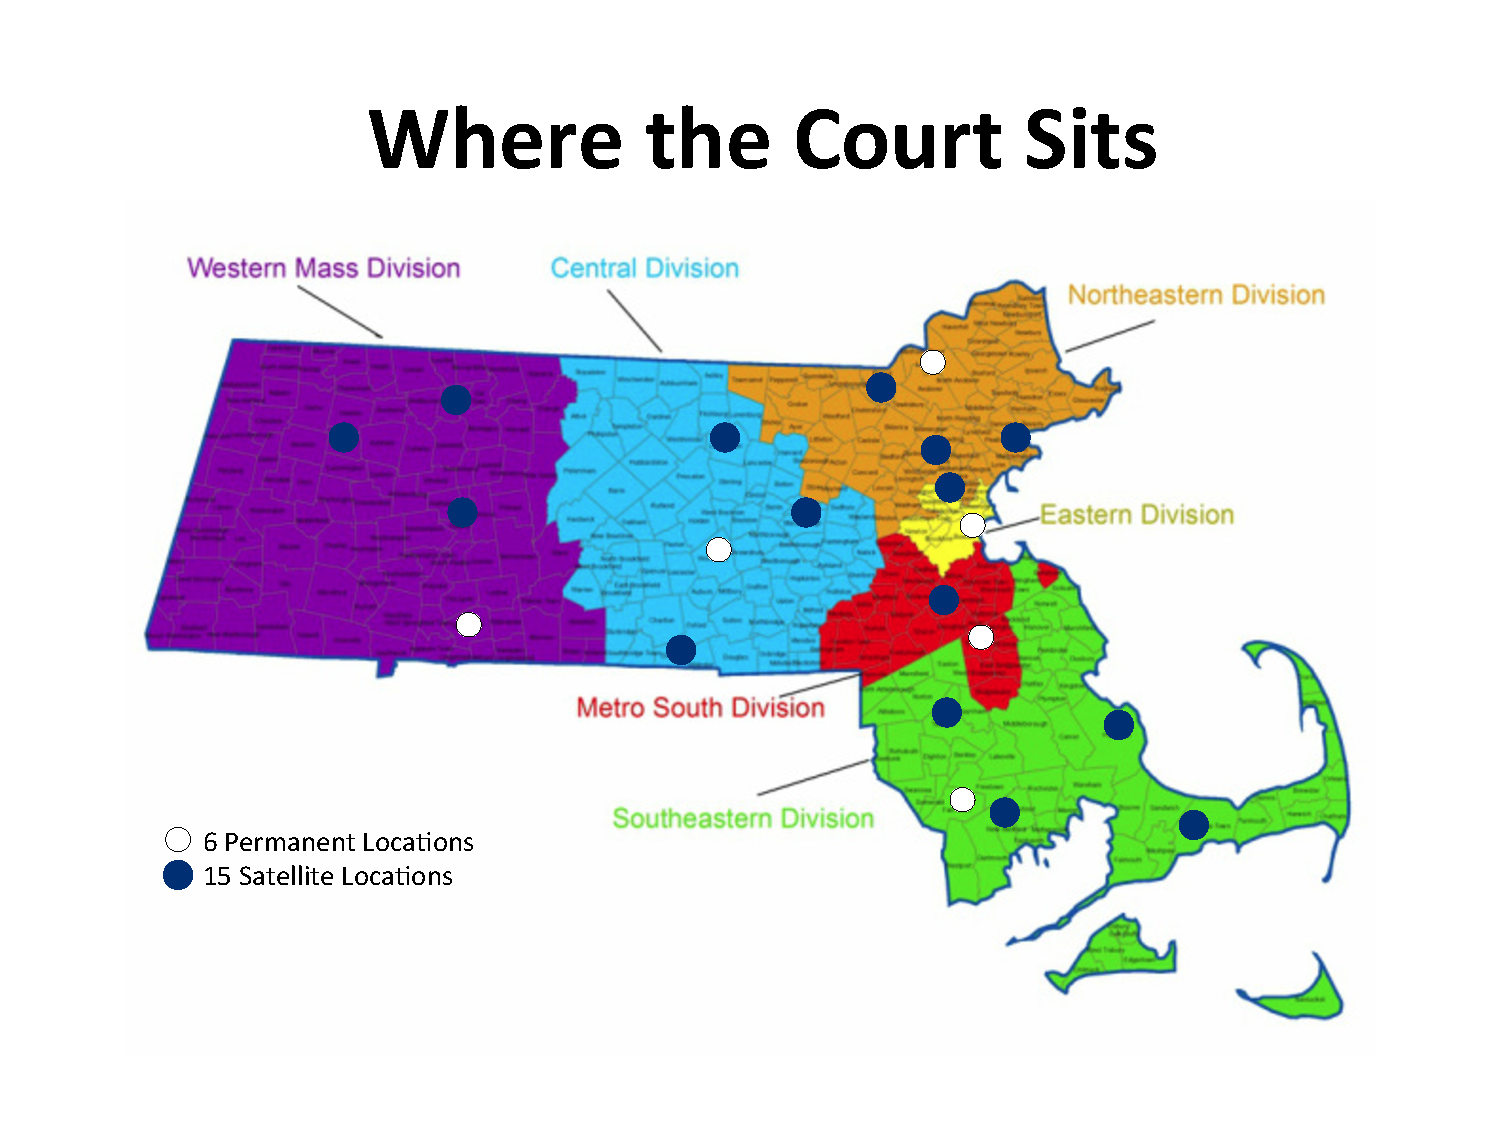
\includegraphics{research/institutional_context/sources/map_of_where_court_sits_-_jan_2019.pdf}
            \caption{Divisions of the Massachusetts Housing Court}
        \end{figure}
        
        
        Four features distinguish the Housing Court as a legal institution from the District Court and Boston Municipal Court \citep{noauthor_housing_nodate}. First, it is led by justices with significant knowledge and experience when it comes to housing-related legal matters, such as summary process cases. Second, it is staffed by housing specialists, employees of the Court with detailed knowledge of Massachusetts housing law who provide information and referrals to resources for landlords and tenants. Third, it offers a service known as mediation, in which cases may be resolved prior to arguments in front of a judge. Mediation is facilitated by a housing specialist, who helps the defendant and plaintiff come to an agreement and records promises made by both sides. Rather than risk defeat at the hands of a judge, many tenants and landlords prefer to reach mutually agreeable terms of resolution during mediation. If either party violates the terms of the specified mediation agreement, the other may return to the judge in a more favorable legal position. Fourth, either party in a summary process case filed in District Court or Boston Municipal Court has the right to transfer the case to the Housing Court at any time prior to trial . For these reasons, tenant advocacy groups and landlord associations alike in Massachusetts generally recommend filing summary process cases in the Housing Court \citep{noauthor_massachusetts_nodate, noauthor_housing_nodate}.

        
        \subsubsection{The Eviction Process}
        Tenants in Massachusetts can rent from landlords under the terms of a lease or without one. If a tenant is renting from a landlord without a lease, their tenancy is \textit{at will}. The nature of the agreement between the tenant and the landlord—the \textit{landlord-tenant agreement}—determines the steps that the landlord must take to evict the tenant.

        
        A landlord in Massachusetts begins the eviction process by serving her tenant with a \textit{notice to quit}, which serves as written notice of her desire to terminate tenancy. While a landlord may deliver the notice to quit herself, many landlords choose to hire a local law enforcement officer to do so for around 40 dollars. This guarantees that an independent third party can vouch that the notice was properly served. A notice to quit is served for \textit{nonpayment of rent}, \textit{cause}, or \textit{no fault} and gives an amount of time after which the landlord-tenant agreement will be terminated if no action is taken by the tenant.
        
        If the notice to quit is served for nonpayment of rent, then regardless of the nature of the landlord-tenant agreement, this time period given by the notice to quit is 14 days. The tenant may \textit{cure} the nonpayment of rent, nullifying the notice to quit, by paying the landlord all owed rent with interest and costs within 14 days \footnote{Tenants at-will do not have the option to cure nonpayment of rent if they have received a separate notice to quit for nonpayment of rent during the last 12 months.}. If the notice to quit is served for cause and a lease defines the landlord-tenant agreement, then the amount of time that given by the notice to quit must be specified in the lease. If the landlord-tenant agreement is at will, then the time period given by the notice to quit is 30 days. No fault notices to quit waiting period of 30 days or one full rental period—whichever is longer—before tenancy can be terminated. 

        After the length of time specified by the notice to quit has passed \footnote{If the notice to quit was for nonpayment of rent, the specified length of time must pass without curing of the nonpayment by the tenant.}, the tenant's rental agreement has ended. To continue with the eviction, the landlord is required to hire a local law enforcement officer to serve the tenant with a \textit{summary process summons and complaint}. Massachusetts law says that the summary process summons and complaint must then be filed with the court on a Monday between seven and 30 days after it was served. The date on which the summons and complaint is filed with the court is known as the \textit{entry date}. If a landlord fails to follow any of the above protocol—say, by serving a notice to quit that specifies too short of a time period or by failing to deliver a summary process summons and complaint to the tenant—her case may be dismissed, automatically awarding victory to the tenant.

        

        

        
        
        
    \subsection{Crime Incident Responses}

\section{Data} \label{sec:data}

    \subsection{Evictions Data}

        \newpage
        \begin{figure}[H]
            \centering
            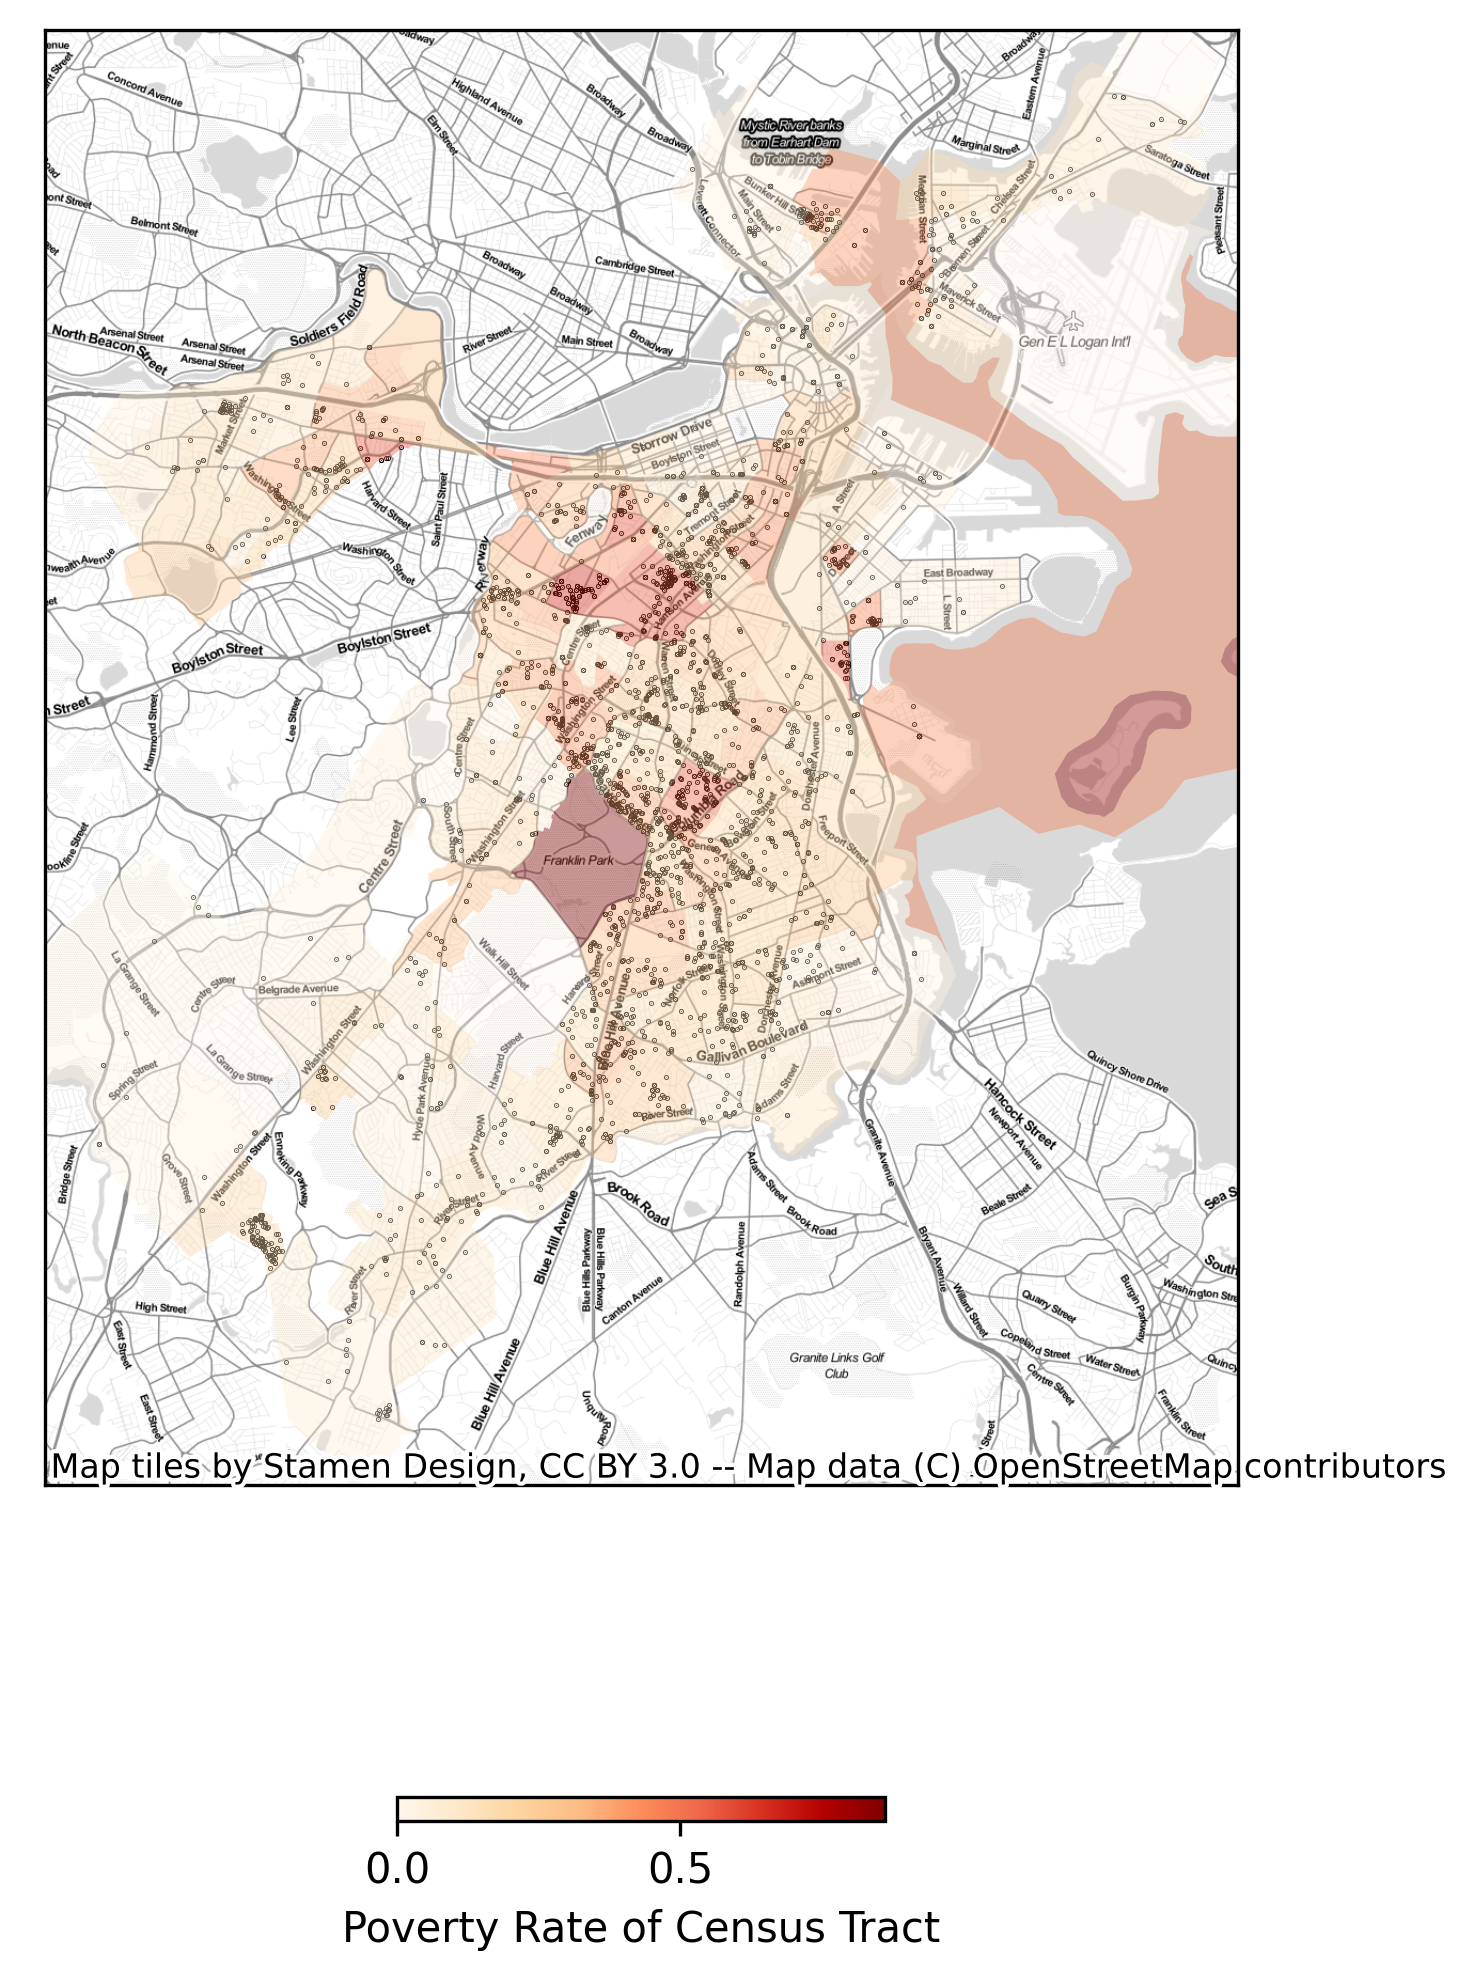
\includegraphics{output/summary_statistics/figures/evictions_map.png}
            \caption{Spatial Incidence of Eviction}
            \label{fig:my_label}
        \end{figure}

        \begin{landscape}
        \begin{figure}[H]
            \centering
            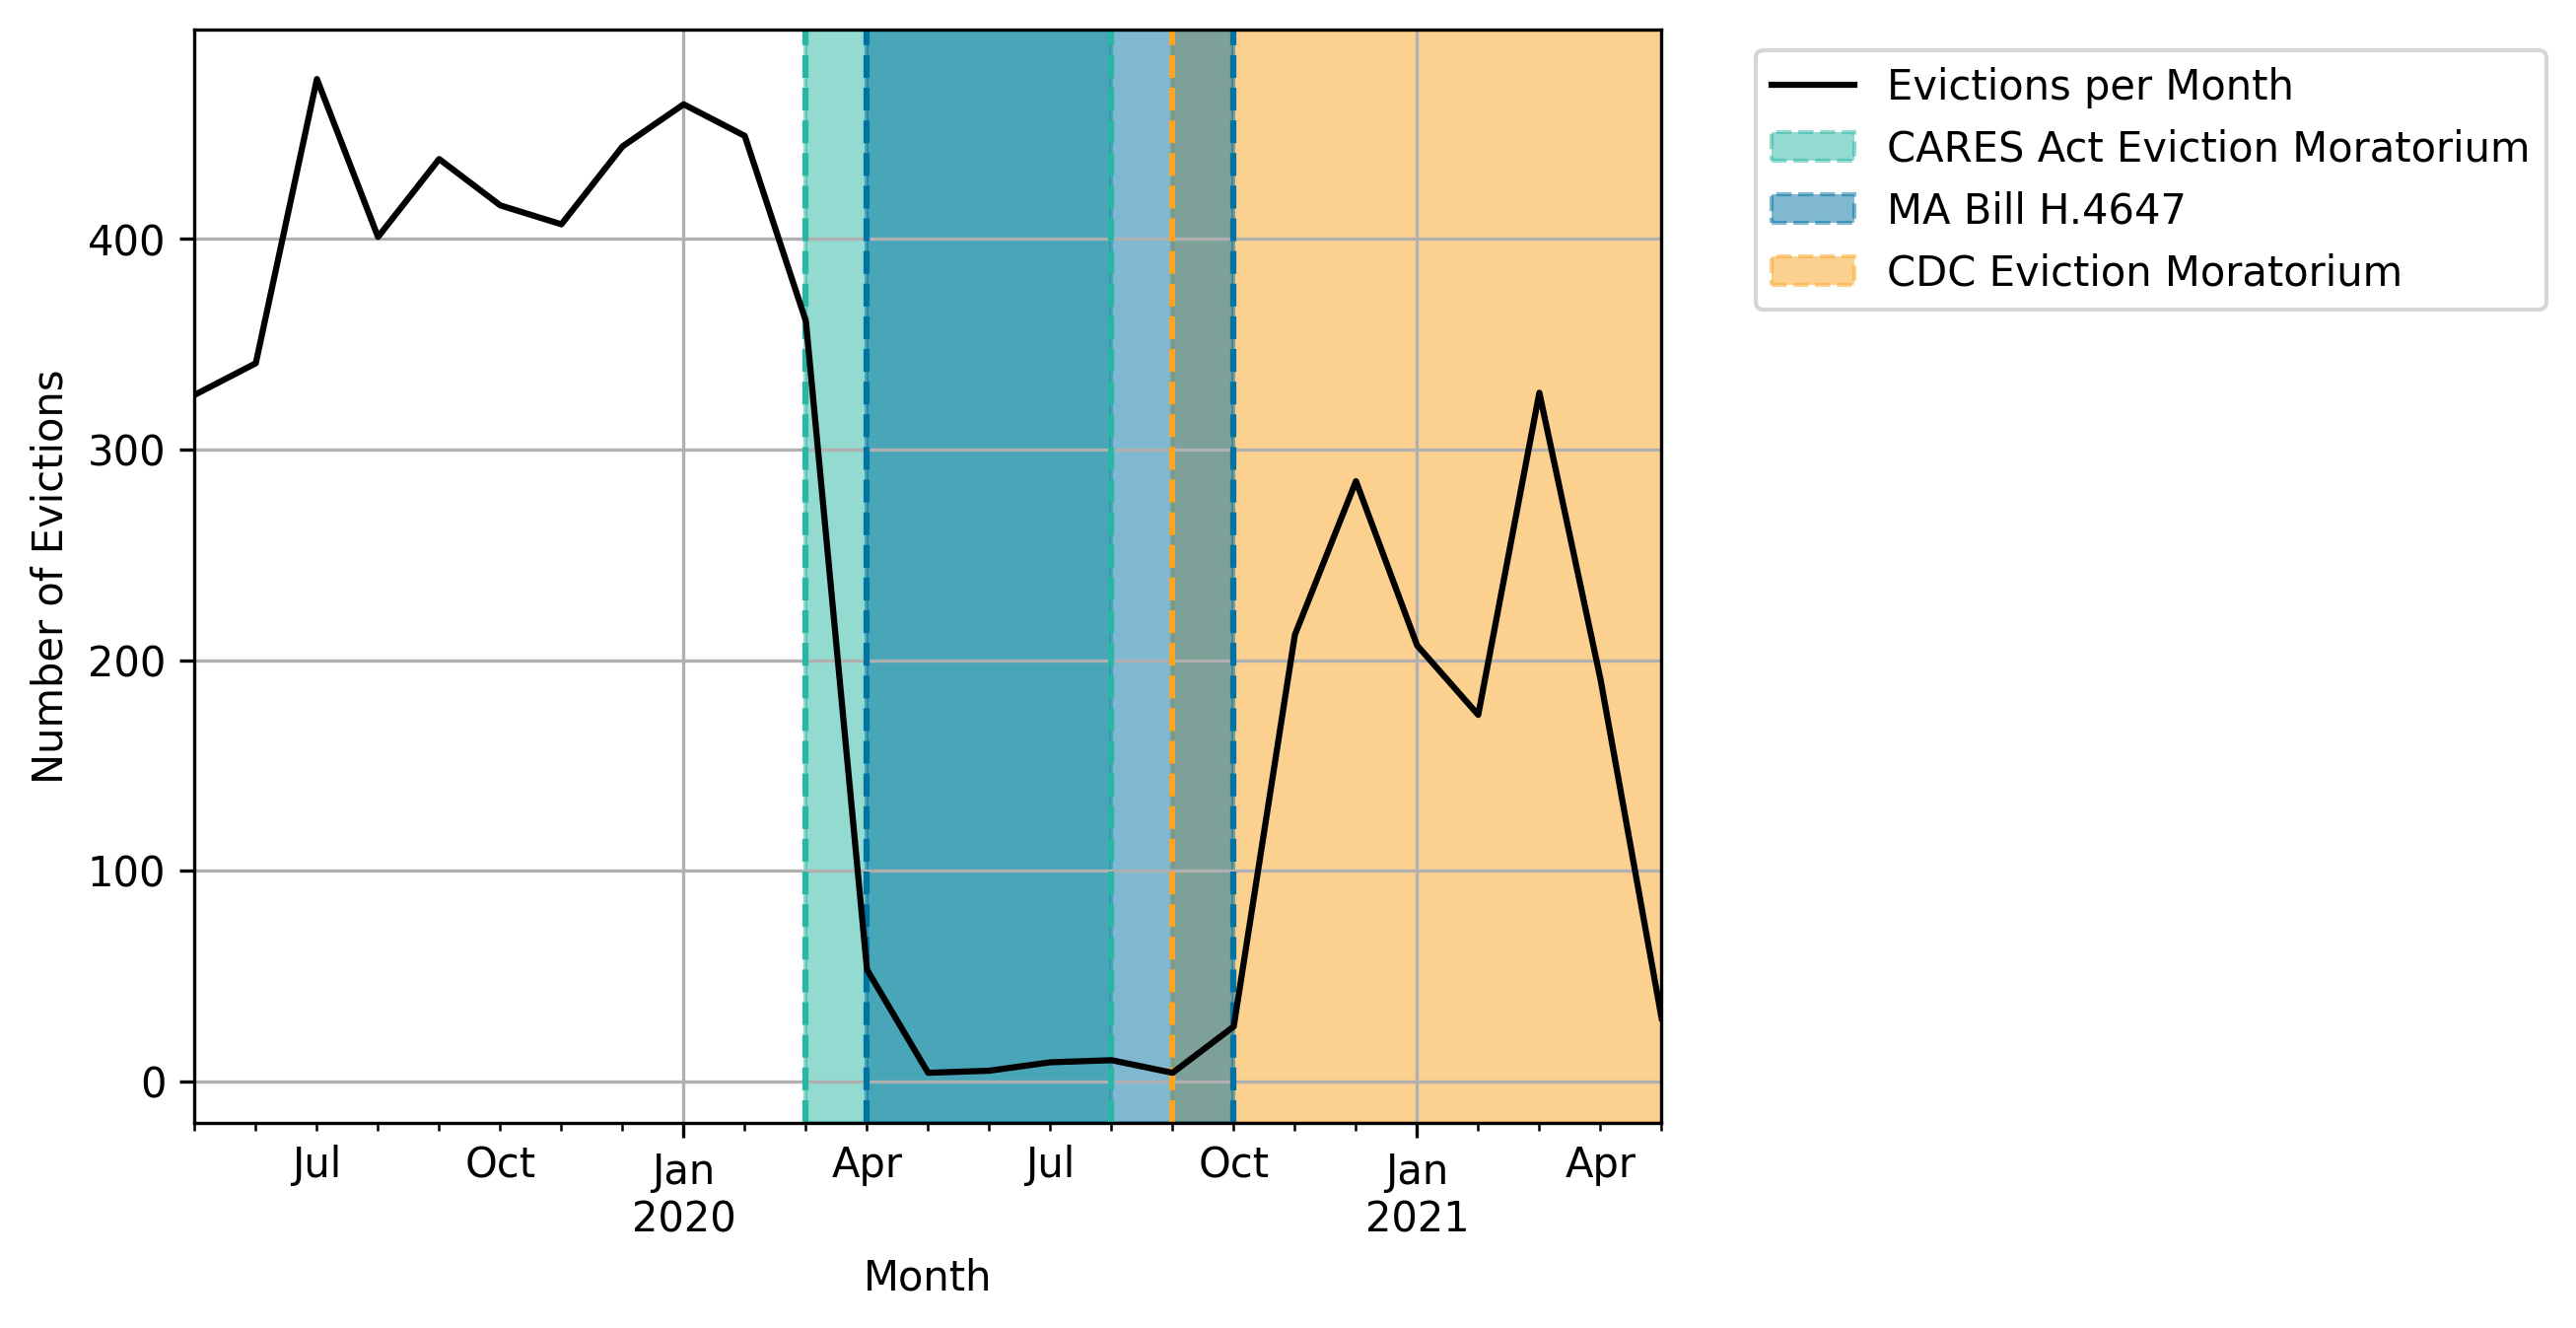
\includegraphics[scale=1.25]{output/summary_statistics/figures/filings_over_time.png}
            \caption{Eviction Filings Over Time in Boston}
            \label{fig:my_label}
        \end{figure}
\end{landscape}
        \begin{table}[H]
            \centering
            \small
            \begin{tabular}{lccc}
\toprule
 & Cases Won By Defendant & Cases Won By Plaintiff & Portion of All Cases \\
\midrule
All Filing Dates & 858 & 2,440 & 1.00 \\
2019-05 & 100 & 156 & 0.08 \\
2019-06 & 38 & 151 & 0.06 \\
2019-07 & 42 & 198 & 0.07 \\
2019-08 & 31 & 178 & 0.06 \\
2019-09 & 37 & 156 & 0.06 \\
2019-10 & 33 & 148 & 0.05 \\
2019-11 & 23 & 138 & 0.05 \\
2019-12 & 28 & 171 & 0.06 \\
2020-01 & 17 & 159 & 0.05 \\
2020-02 & 38 & 139 & 0.05 \\
2020-03 & 70 & 85 & 0.05 \\
2020-04 & 14 & 19 & 0.01 \\
2020-05 & 0 & 1 & 0.00 \\
2020-06 & 2 & 2 & 0.00 \\
2020-07 & 1 & 2 & 0.00 \\
2020-08 & 1 & 2 & 0.00 \\
2020-09 & 1 & 6 & 0.00 \\
2020-10 & 7 & 14 & 0.01 \\
2020-11 & 54 & 151 & 0.06 \\
2020-12 & 71 & 159 & 0.07 \\
2021-01 & 81 & 120 & 0.06 \\
2021-02 & 58 & 86 & 0.04 \\
2021-03 & 58 & 89 & 0.04 \\
2021-04 & 45 & 93 & 0.04 \\
2021-05 & 8 & 17 & 0.01 \\
\bottomrule
\end{tabular}

            \caption{Distribution of Eviction Filings and Outcomes}
            \label{tab:my_label}
        \end{table}


    \subsection{Summary Statistics}
         \begin{table}[H]
            \centering
            \small
            \begin{tabular}{llcccc}
\toprule
 &  & Mean & Median & S.D. & N \\
Panel & Variable &  &  &  &  \\
\midrule
\multirow[c]{3}{4cm}{\textit{Panel A: Case Initiation}} & For cause & 0.12 & 0.00 & 0.33 & 40,727 \\
 & No cause & 0.11 & 0.00 & 0.31 & 40,727 \\
 & Non-payment of rent & 0.75 & 1.00 & 0.43 & 40,727 \\
\cline{1-6}
\multirow[c]{6}{4cm}{\textit{Panel B: Case Resolution}} & Case defaulted & 0.20 & 0.00 & 0.40 & 40,727 \\
 & Case dismised & 0.29 & 0.00 & 0.45 & 40,727 \\
 & Case duration & 57.81 & 21.00 & 78.29 & 39,087 \\
 & Case heard & 0.06 & 0.00 & 0.23 & 40,727 \\
 & Case mediated & 0.41 & 0.00 & 0.49 & 40,727 \\
 & Money judgment & 1,890.34 & 0.00 & 5,279.49 & 40,727 \\
\cline{1-6}
\multirow[c]{4}{4cm}{\textit{Panel C: Defendant and Plaintiff Characteristics}} & Defendant has an attorney & 0.09 & 0.00 & 0.28 & 40,727 \\
 & Defendant is an entity & 0.01 & 0.00 & 0.08 & 40,727 \\
 & Plaintiff has an attorney & 0.84 & 1.00 & 0.37 & 40,727 \\
 & Plaintiff is an entity & 0.70 & 1.00 & 0.46 & 40,727 \\
\cline{1-6}
\multirow[c]{4}{4cm}{\textit{Panel D: Assessor Records From Most Recent Pre-Filing F.Y.}} & Building value & 8,350,204.19 & 636,500.00 & 22,073,916.94 & 36,587 \\
 & Land value & 2,471,065.61 & 192,400.00 & 6,218,383.08 & 36,587 \\
 & Other value & 112,575.80 & 1,000.00 & 659,661.29 & 36,587 \\
 & Total property value & 10,900,678.30 & 954,900.00 & 26,482,630.60 & 36,587 \\
\cline{1-6}
\multirow[c]{4}{4cm}{\textit{Panel E: Census Tract Characteristics}} & Median household income (2016) & 52,659.44 & 47,105.00 & 27,177.48 & 40,726 \\
 & Median two bedroom rent (2015) & 1,116.27 & 1,055.00 & 396.29 & 30,537 \\
 & Population density (2010) & 9,159.77 & 5,978.61 & 9,574.14 & 40,726 \\
 & Portion white (2010) & 0.58 & 0.63 & 0.29 & 40,726 \\
\cline{1-6}
\multirow[c]{9}{4cm}{\textit{Panel F: Zestimates Around Filing Date}} & Filing date & 377,384.02 & 305,144.00 & 316,645.29 & 10,096 \\
 & Five years before filing date & 261,462.86 & 213,270.60 & 238,040.64 & 9,842 \\
 & Four years before filing date & 280,243.32 & 225,065.75 & 276,051.45 & 9,968 \\
 & One year after filing date & 421,601.75 & 347,550.00 & 344,328.86 & 10,443 \\
 & One year before filing date & 351,172.05 & 278,722.25 & 311,982.74 & 10,190 \\
 & Three years after filing date & 501,611.80 & 414,600.00 & 780,467.01 & 5,894 \\
 & Three years before filing date & 307,137.16 & 240,097.38 & 369,763.53 & 10,172 \\
 & Two years after filing date & 477,948.08 & 393,900.00 & 457,694.83 & 9,175 \\
 & Two years before filing date & 341,084.08 & 259,176.00 & 987,145.51 & 10,182 \\
\cline{1-6}
\bottomrule
\end{tabular}

            \caption{Summary Statistics}
            \label{tab:table_1}
        \end{table}
        \newpage

\section{Empirical Strategy: Difference-in-Differences}
    I seek to estimate the average treatment effects of plaintiff victory in eviction cases on treated properties. I use the staggered difference-in-difference estimator proposed in \cite{callaway_difference--differences_2021}, which uses two-period, two-unit difference-in-difference estimators to estimate time- and cohort-specific ATTs and then aggregates them, weighting by cohort size, to produce summaries of the ATT. 
    
    
    Let $G_i$ be the month during which the eviction case involving property $i$ was filed, such that $G_i = g \in \{\text{May} \; 2019, \text{June} \; 2019, ..., \text{May} \; 2021\}$. Let $C_i = 1$ if the eviction case involving $i$ resulted in a victory for the defendant and $0$ otherwise. If $G_i = g$ and $C_i = 0$, then property $i$ is a treated property and a member of the cohort first treated during month $g$ (cohort $g$). If $C_i=1$, then property $i$ is a never-treated property. Let $Y_{i,t}$ be property $i$'s Zestimate during month $t$ and define $\Delta Y_{i, g-1, t} \equiv Y_{i,t} - Y_{i,g-1}$ so that $\Delta Y_{i, g-1, t}$ is the change in property $i$'s Zestimate between months $t$ and $g-1$.

    \subsection{Unconditional Estimates of the ATT}
    The following is an unconditional estimator for $ATT(g,t)$, the average treatment affect during month $t$ for cohort $g$.
    \begin{align}
        \hat{ATT}^{nev}_{un}(g, t) = \frac{\sum_i\Delta Y_{i, g-1, t}\mathds{1}\{G_i=g\}}{\sum_i\mathds{1}\{G_i=g\}} - \frac{\sum_i\Delta Y_{i, g-1, t}\mathds{1}\{C_i=1\}}{\sum_i\mathds{1}\{C_i=1\}}
    \end{align}
    The above estimator will identify $ATT(g,t)$ under the assumption that the change in untreated potential outcomes between periods $g-1$ and $t$ is the same among units in cohort $g$ as it is among never-treated units.

    \subsection{D.R. Estimates of the ATT}

    The above unconditional parallel trends assumption is unlikely to hold, as eviction case outcomes and zestimates may be related to their socioeconomic surroundings. Table 3 explores this theory further, reporting results from univariate regressions of January 2022 Zestimates and an indicator for plaintiff victory on the pre-treatment characteristics listed in Panels A through D of Table 2. Each cell gives the p-value from a regression of the variable which labels its column on the variable which labels its row. Table 3 shows significant associations between pre-treatment characteristics and Zestimates and pre-treatment characteristics and case outcomes, suggesting that the unconditional parallel trends assumption imposed earlier may not be valid.

    \begin{table}[H]
        \centering
        \input{}
        \caption{Relationship Between Pre-Treatment Characteristics and the Dependent and Independent Variables}
        \label{tab:my_label}
    \end{table}

    My next strategy uses covariates to construct a more credible counterfactual for the observed path of outcomes in the treatment group using the doubly robust difference-in-differences estimator proposed by \cite{santanna_doubly_2018}. For each property, let $X_i$ be a vector containing the covariates whose univariate regression coefficients from column 1 of table 3 are significant at the 5 percent level. To attempt to identify $ATT(g, t)$ using the doubly robust estimator, I first estimate $\hat{p}_g(X_i)$, a logit regression propensity score model for being in cohort $g$. I assign a weight $\hat{w}_i(X_i) \equiv\frac{\hat{p}_g(X_i)}{1 - \hat{p}_g(X_i)}$ to each never-treated property $i$; $\hat{w}_i(X_i) \equiv 1$ for treated properties. Define $\hat{w}^*_i(X_i) = \frac{\hat{w}_i(X_i)}{\sum_i \hat{w}_i(X_i)}$. Second, using only never-treated counties, I regress $\Delta Y_{i, g-1, t}$ on $X_j$, weighting by $\hat{w}_i(X_i)$. Using the estimated coefficients $\hat{\beta}_{g-1, t}^{X}$, I define $\Delta \hat{\mu}_{g-1, t}(X_i) \equiv \hat{\beta}_{g-1, t}^{X}X_i$ so that $\Delta \hat{\mu}_{g-1, t}(X_i)$ is the predicted change in property $i$'s Zestimate between months $t$ and $g-1$.
    The doubly robust estimator for $ATT(g, t)$ is as follows.
    \begin{align}
        \hat{ATT}^{nev}_{DR, X}(g,t) = \frac{1}{N}\sum_i[(\frac{D_i}{\Bar{D_i}} - \frac{\hat{w}^*_i(X_i)C_i}{\Bar{C_i}})(\Delta Y_{i, g-1, t} - \hat{\mu}_{g-1, t}(X_i))]
    \end{align}
    Note that $\Bar{D_i}$ and $\Bar{C_i}$ are sample averages. Under the assumption of parallel trends among units with the same covariates, $\hat{ATT}^{nev}_{DR, X}(g,t)$ will identify $ATT(g, t)$.
    

    Columns 2 and 3 of table 4 shows significant pre-treatment imbalance in covariates between the treatment and control groups. Each row of column 2 reports the coefficient from a univariate regression of one covariate on an indicator for plaintiff victory. Column 3 reports the p-values associated with each of these coefficients. In each row of column 4, I regress one covariate on an indicator for plaintiff victory and $\hat{w}_i(X_i)$ and report the coefficient on the indicator for plaintiff victory. Column 5 reports the p-values associated with each coefficient and shows that conditioning on pre-treatment covariates makes virtually all pre-treatment differences in covariates insignificant.

    The estimator defined in equation 2 simultaneously models the counterfactual change in \emph{observed} outcomes for untreated properties ($\hat{w}_i(X_i)$) and the \emph{predicted} change in outcomes for untreated properties ($\hat{\mu}_{g-1, t}(X_i)$). As long as one of these two models is correctly specified, the doubly robust estimator will identify $ATT(g, t)$.

    \newpage
    \begin{landscape}
       \begin{table}[H]
        \centering
        \input{}
        \caption{Balance Tests}
        \label{tab:my_label}
    \end{table} 
    \end{landscape}

    \subsection{Aggregating Treatment Effects Across Cohort and Time}
        \subsubsection{ATTs Across Cohorts}
        \subsubsection{ATTs Across Time Periods}
        \subsubsection{Event-Study ATTs}
    
\section{Results} \label{sec:result}

    \subsection{Unconditional Estimates of the ATT}

 

    \subsection{D.R. Estimates of the ATT}


    


\section{Conclusion} \label{sec:conclusion}


\bibliography{citations}


\clearpage

\onehalfspacing

%
\end{document}